\documentclass[a4paper,12pt]{article}

\usepackage[top = 2.5cm, bottom = 2.5cm, left = 2.5cm, right = 2.5cm]{geometry} 
\usepackage{CJKutf8}
\usepackage[T1]{fontenc}
\usepackage[utf8]{inputenc}
\usepackage{multirow} 
\usepackage{booktabs}
\usepackage{enumitem}
\setitemize{noitemsep,topsep=0pt,parsep=0pt,partopsep=0pt}
\renewcommand{\labelitemi}{$\diamond$}
\usepackage{listings}
\usepackage{xcolor}
\usepackage{graphicx}
\usepackage{caption}
\usepackage{setspace}
\setlength{\parindent}{0in}
\usepackage{float}
\usepackage{fancyhdr}
\pagestyle{fancy}
\fancyhf{}
\setlength{\headheight}{16pt}
\newcommand{\selfjp}{\begin{CJK*}{UTF8}{min}ドゥーマ\end{CJK*}}
\newcommand{\source}[1]{\caption*{Source: {#1}} }
\newcommand{\htmlelem}[1]{\lstinline[columns=fixed,language=HTML]{#1}}
\newcommand{\nsp}{\vspace{0.05cm}\\}
\lhead{\footnotesize Web Development: Lesson 1}
\rhead{\footnotesize Doomer / \selfjp}
\cfoot{\footnotesize \thepage} 

\definecolor{codegreen}{rgb}{0,0.6,0}
\definecolor{codegray}{rgb}{0.5,0.5,0.5}
\definecolor{codepurple}{rgb}{0.58,0,0.82}
\definecolor{backcolour}{rgb}{0.95,0.95,0.92}
\lstdefinestyle{mystyle}{
    backgroundcolor=\color{backcolour},   
    commentstyle=\color{codegreen},
    keywordstyle=\color{magenta},
    numberstyle=\tiny\color{codegray},
    stringstyle=\color{codepurple},
    basicstyle=\ttfamily\footnotesize,
    breakatwhitespace=false,         
    breaklines=true,                 
    captionpos=b,                    
    keepspaces=true,                 
    numbers=left,                    
    numbersep=5pt,                  
    showspaces=false,                
    showstringspaces=false,
    showtabs=false,                  
    tabsize=2
}
\lstset{style=mystyle}

\begin{document}

\thispagestyle{empty} 

\begin{tabular}{p{15.5cm}} 
{\large \bf Web Development: Lesson 1} \\
Discord Lessons\\ Fall 2020\\ Doomer / \selfjp \\
\hline
\\
\end{tabular}

\vspace*{0.3cm}

\begin{center}
	{\Large \bf Lesson 1 - The Hypertext Markup Language}
	\vspace{2mm}\\
	{\bf dedicated to Spennorex and Grumpah}
		
\end{center}  

\vspace{0.4cm}

\section{Introduction}
In this lesson we'll learn the most important terms of web development, which might be used later on to explain more complex concepts and build a basic web page. This guide is meant to be for complete beginners and can therefore be skipped by people, who already feel comfortable with HTML. As a side note: if you want to follow along this script, you'll see passages where code snippets are included. In order to get those running you need to create a text file with your preferred editor and paste / write the code inside the file, after having done that you need to change the file extension from ".txt" to ".html" and then you can simply save and double-click to open it in your browser. Don't be worried if something is not working properly, feel free to drop me a message (Doomer\#1718).

\section{Document Structure}
In order to create a web page, we need to understand the language web documents are written in - \textbf{HTML} (Hyper Text Markup Language). This language is used to describe the \textbf{DOM} (Document Object Model) of a web page. To get a better grasp of the concept, here's an illustration:

\begin{figure}[h]
    \centering
    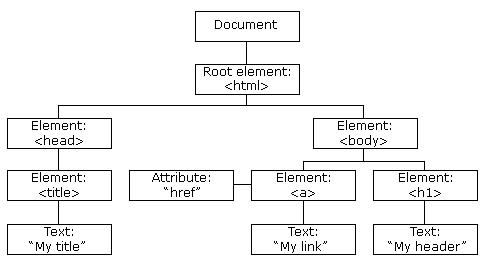
\includegraphics[width=0.75\textwidth]{imgs/dom-tree}
    \caption{HTML DOM}
    \label{fig:dom-tree}
    \source{https://www.w3schools.com/js/pic\_htmltree.gif}
\end{figure}

It might be confusing in the beginning, but that's how a web page looks like for a browser. This particular example, would look like this, if we'd code it:

\begin{lstlisting}[language=HTML,caption=DOM Example Page,label={lst:sample_1}]
<html>
    <head>
        <title>My title</title>
    </head>
    <body>
        <a href>My link</a>
        <h1>My header</h1>
    </body>
</html>
\end{lstlisting}

If you look at this snippet, you might see some interesting things. There are words inside brackets, also called \textbf{tags}. The one without the '/' is called \textbf{start tag} and the one with '/' is the \textbf{end tag}. These are used to delimit an \textbf{element}.\\ 
Everything inside those tags is considered to be an html element, additionaly one should add as seen in the example, that an element can contain other elements. In Listing \ref{lst:sample_1} you can see, that the "html" element contains the "head" and the "body" elements, which themselves contain the "title" and the "a" and "h1" elements.\\
Now that we have covered what elements are, we can look into learning a few html-elements, to get a basic "vocabulary".

\section{HTML Elements}
You've already seen following elements:
\begin{itemize}
    \item \htmlelem{<html>}
    \item \htmlelem{<head>}
    \item \htmlelem{<body>}
    \item \htmlelem{<title>}
    \item \htmlelem{<a>}
    \item \htmlelem{<h1>}
\end{itemize}
Let's first discuss the first three elements. Those three are called the \textbf{Document structure elements} - they organize the huge document into compartments.\nsp
The \htmlelem{<html>} element is the root element and contains every other element, that's why it's common to see a \htmlelem{<html>} at the beginning of an html-file and a \htmlelem{</html>} at the end of it.\nsp
The \htmlelem{<head>} element is the meta information element and contains information you don't see on the page itself, such as the title.\nsp
The \htmlelem{<body>} element is the place where the actual content belongs to - the text that is displayed on the web page.\vspace{0.15cm}\nsp
Next we have the elements that can be used inside the \htmlelem{<head>}, those are called \textbf{Document head elements}, these include:\nsp
The \htmlelem{<title>} element is used to define the page title and is what you usually the browser tab name.\nsp
There are a few other important ones, which we'll cover as soon as we need them.\vspace{0.15cm}\nsp
The contents of \htmlelem{<body>} are called the \textbf{Document body elements} and manage the content of the page. We'll start of with the simplest element.\nsp
The \htmlelem{<p>} element is used to define a \underline{p}aragraph of text. This is where you could put a simple text. If you want to have a new line (line break) inside the text (applies to any html element) you need to insert this \textbf{self-closing} tag \htmlelem{<br/>}. If you see a tag, which has the '/' at the end it means that it is \textit{self-closing}, thus you don't have to have 2 tags as usual - one for the opening, one for the closing, but one.\nsp
The familiar \htmlelem{<h1>} is a \underline{h}eading element and the 1 means that it is a top layer heading, which makes the text huge, in html you can have up to 6 levels of headings - from \htmlelem{<h1>} to \htmlelem{<h6>}, where an increasing number means a decreasing font-size.\nsp
Another common html elements are the list elements \htmlelem{<ul>} for \underline{u}nordered \underline{l}ists and \htmlelem{<ol>} for \underline{o}rdered \underline{l}ists, where the unordered is using bullet points for its items and the ordered arabic numerals (per default). Both lists contain items, which are defined by the \htmlelem{<li>} \underline{l}ist-\underline{i}tem tag.\nsp
The last body tag for now will be the \underline{a}nchor tag \htmlelem{<a>}, which is also shown above - it allows us to insert a link to another web page or our own subpage, we'll look into this later, as soon as we'll start using multiple html files together.
\section{Building our Web Page}
So now that we've covered quite a bit of theory, we can start building a very simple \textit{static} webpage, which will improve a lot over time. To start off we can use the standard wireframe of web pages:
\begin{lstlisting}[language=HTML,caption=Our HTML Wireframe,label={lst:html_wireframe}]
<html>
    <head>
        <title></title>
    </head>
    <body>
    </body>
</html>
\end{lstlisting}
Now it's time to pack some stuff into our skeleton.
\begin{lstlisting}[language=HTML,caption=Content Update,label={lst:html_wireframe_1}]
<html>
    <head>
        <title>My Profile</title>
    </head>
    <body>
        <h1>My Profile Page</h1>
        <p>Here's who I am :)</p>
        <ol>
            <li>Name: Doomer</li>
            <li>How many Discord Notifications do you have? 0</li>
            <li>Gender: genderfluid</li>
            <li>Birthday: 22nd of December</li>
            <li>Timezone: UTC+2 (CET)</li>
            <li>Languages Spoken: English, Russian, German</li>
            <li>Favorite Colors: Black, Blue, Purple</li>
            <li>...</li>
        </ol>
        <p>I think that's enough <br/> for an example.</p>
    </body>
</html>
\end{lstlisting}
I hope that from that example you could understand the basic structure of an html document and therefore can do this yourself. I think I'll end this theoretical part of the script with this, since we covered a lot of different elements and it's probably going to take a while to get everything into your mind. The next update would be covering styling and making the web page look beautiful, which is a huge update, thus I decided to pack it into the next script.

\section{Excercises}
These excercises are optional and you can do them if you want to get experience and feel comfortable using the basic HTML syntax:
\begin{enumerate}
    \item Create a profile page for yourself.
    \item Create a page with your favorite song lyrics.
    \item Create a site with movies / books / anime you watched, with a small description for each
\end{enumerate}

\section{Final Notes}
If any questions occur, you can always ask me (it might take some time, since we are not necessarily in the same timezone), but you'll get an answer. If you can make the excercises without looking back to my templates, then it'd be great, but it's definitely not wrong or bad to use a reference - to be honest, most developers nowadays use a \textit{ton} of copied code, but it's useful to have a foundation to build on. If you're disappointed, that everything was very easy or difficult, give me some feedback! I haven't created scripts that often and mostly have done it for myself, so I have no idea if what I've done is great, ok or absolute garbage, so please if you have anything to criticize - do it! I should add as well that I'm not too good in english, since it's not my mothertongue, so if you see me use some weird formulation / wrong order or literally any other possible mistake, tell me, so I can make this more easy and comfortable to read! Thanks a lot for reading this far :). See you in the next script.

\end{document}
